\begin{refsection}

	\chapter{Aprenentatge automàtic}
	\label{chap:ML}
	
	En el sentit més bàsic, l'aprenentatge automàtic és una manera d'implementar la intel·ligència artificial. De forma similar a l'IA, l’aprenentatge automàtic és una branca de la informàtica en la qual s'estudia el disseny d'algoritmes que puguin aprendre. En l'aprenentatge automàtic s'utilitzen algoritmes que proporcionen a l'ordinador la capacitat d'aprendre i comprendre automàticament sense haver de ser programat una vegada darrere l'altra.
	
	Com aprendrà l'ordinador de forma automàtica? Amb les dades. S'introdueixen les dades amb diferents atributs o característiques a partir de les quals els algoritmes han d'entendre i fer prediccions en funció de les dades proporcionades. Una vegada que l'algoritme ha après i interpretat les dades, és a dir, que s’ha format per si mateix, es posar l'algoritme a prova i sense programar-les explícitament, introduir dades de prova i obtenir resultats.

	\section{Aprenentatge supervisat}
	
	L'aprenentatge supervisat, com el seu nom indica, és una tècnica d'aprenentatge on es supervisa o es controla tot el procés d’aprenentatge. L'objectiu principal d'aquests algoritmes d'aprenentatge és predir el resultat d'un conjunt de mostres d'entrenament juntament amb les etiquetes (resultats desitjats) de mostres. Durant l'entrenament l'algoritme sap el que hauria de predir, per això s'anomena aprenentatge supervisat.\supercite{DataCamp}
	
	Suposem que tenim 10000 imatges, 5000 imatges de gats i 5000 de gossos, i cada imatge té una etiqueta: 0 per als gats i 1 per als gossos. L'objectiu d'aquesta tècnica és trobar patrons a les dades donades segons les etiquetes. L’algoritme d’aprenentatge supervisat intentarà trobar un límit entre les 10000 imatges que les divideix en dues parts segons l'etiqueta. De manera que en un moment de prova quan una nova imatge, per exemple una imatge d'un gat es presenta com a entrada sense cap etiqueta, l'algoritme li posarà l'etiqueta 0, cosa que significa que l'algoritme pot predir o classificar aquesta imatge com a imatge d'un gat.\supercite{edureka}
	
	\section{Aprenentatge no supervisat}
	
	A diferència de l’aprenentatge supervisat, els algoritmes d'aprenentatge no supervisat prenen un conjunt de dades que conté només les entrades, sense les etiquetes. Per tant, els algorismes aprenen de les dades que no han estat etiquetades ni classificades.\supercite{mlwiki}
	
	Els algoritmes s'elaboren de tal manera que puguin trobar l'estructura i els patrons adequats en les dades. Una vegada aquests patrons consistents es fan evidents, els punts  similars es poden agrupar junts, i diferents punts estaran en diferents grups. Una aplicació de l’aprenentatge no supervisat es troba en el camp de l’estimació de la densitat en l'àmbit d'estadística amb finalitat de visualització o anàlisi.\supercite{DataCamp}
	
	\section{Aprenentatge per reforç}
	
	L'aprenentatge per reforç és un tipus d’aprenentatge automàtic que té un agent (per exemple, un robot) que aprèn a comportar-se en un entorn fent accions i quantificant els resultats. Si l'agent realitza una resposta correcta, obtindrà un punt de recompensa, fet que augmenta la confiança de l'agent per dur a terme més accions d'aquest tipus. El funcionament d'aquests algoritmes es basa en el procés de decisió de Markov.\supercite{mlwiki,TDSmarkov}
	
	Per exemple, a la \cref{fig:rein}, es pot veure que l’agent (robot) actua en l’entorn (un laberint), interpretant amb els ulls, obté una recompensa per cada moviment correcte i en funció del seu estat actual efectua la següent acció.
	
	Algunes aplicacions de l'aprenentatge per reforç són jugar a jocs (Alpha Go, Escacs, Mario), robòtica, sistemes de control de semàfors, etc.
	
	\begin{figure}[H]
		\centering
		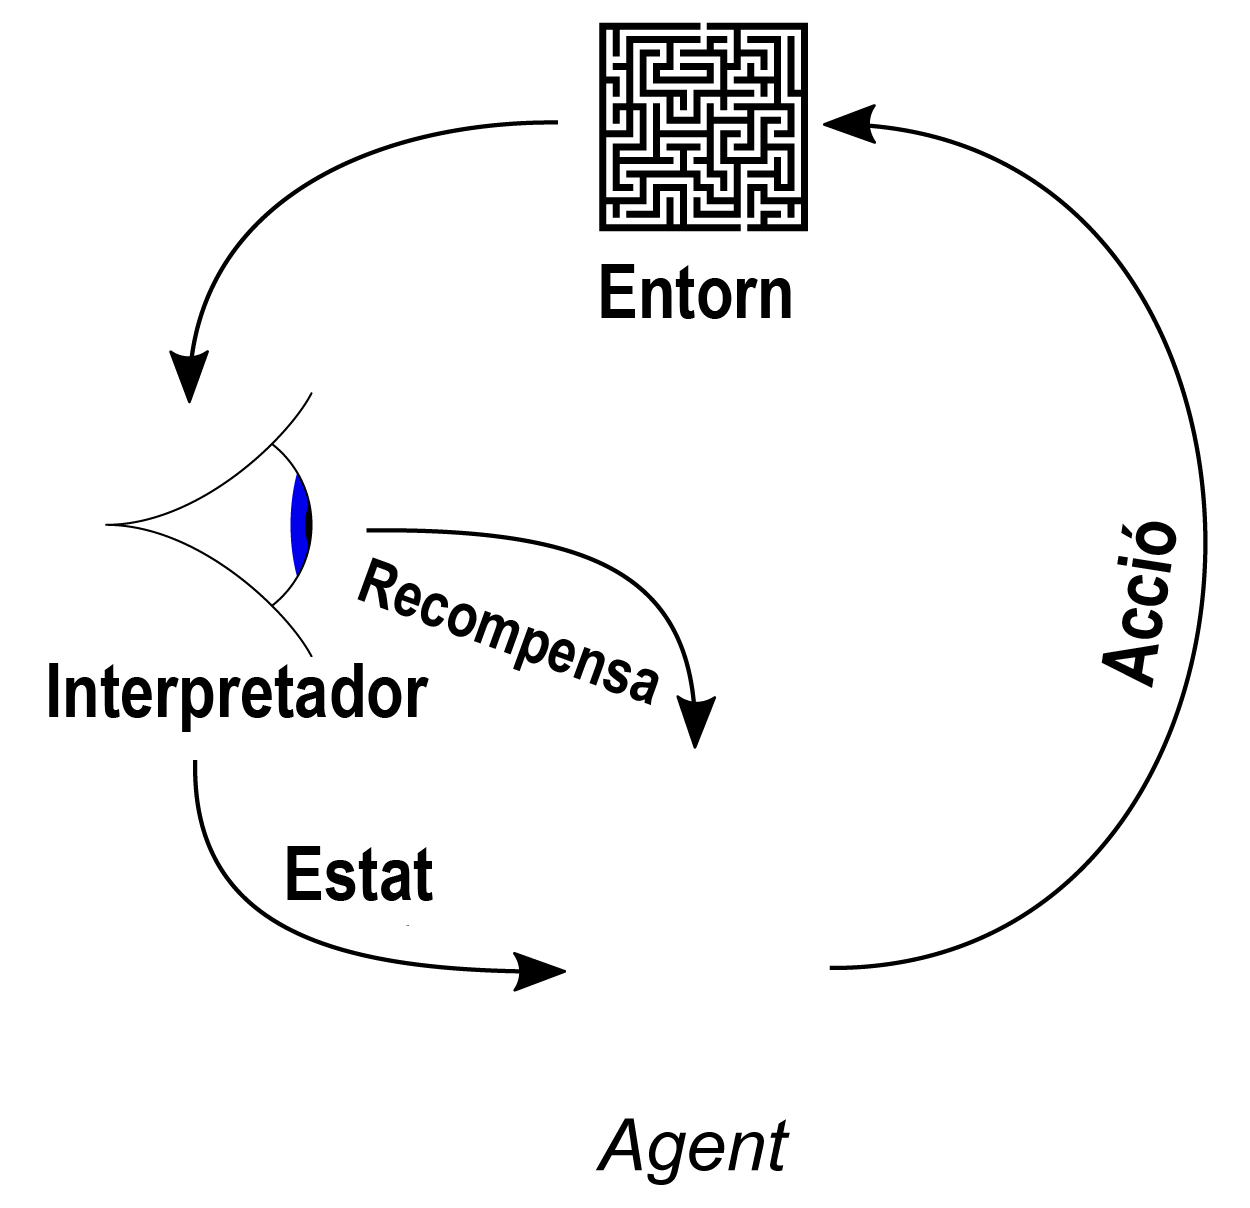
\includegraphics[width=8cm]{Reinforcement}
		\caption{Aprenentatge per reforçament}
		\label{fig:rein}
	\end{figure}
	
	\section{Aprenentatge profund}
	
	L'aprenentatge profund és una subcategoria d'aprenentatge automàtic. De forma similar a l'aprenentatge automàtic, l'aprenentatge profund també té l'aprenentatge supervisat, no supervisat i per reforç. Com s'ha comentat anteriorment, la idea de la IA es va inspirar en el cervell humà. Per tant, l’aprenentatge profund es va inspirar en xarxes neuronals artificials i les xarxes neuronals artificials es van inspirar en xarxes neuronals biològiques humanes. L'aprenentatge profund és una de les maneres d’executar l'aprenentatge automàtic.\supercite{DataCamp,dl}
	
	L'aprenentatge profund utilitza xarxes neuronals artificials amb diverses capes ocultes (\cref{fig:ann}) per extreure progressivament característiques o atributs de nivell superior a partir l’entrada. Per exemple, en el processament d’imatges, les capes inferiors poden identificar les vores, mentre que les capes superiors poden identificar els conceptes rellevants per a un humà com ara dígits, lletres o cares.\supercite{dlwiki}

	\addtocontents{toc}{\vspace{1em}}
	\printbibliography[heading=subbibintoc]

\end{refsection}
